\documentclass{report}

\usepackage[margin=1in]{geometry}
\usepackage{amsmath,amssymb}
%\usepackage{dsfont} %install texlive-fonts-extra 
\usepackage{tikz}
\usetikzlibrary{bayesnet}
\usepackage{setspace}

\author{Otto Fabius}
\title{SGVB Topic Modeling}
\begin{document}
\large
\doublespacing
\maketitle
\begin{abstract}
	content...
\end{abstract}
\chapter*{}
\onehalfspacing
\section*{List of Symbols}
We use lowercase bold-faced symbols to denote vectors, and uppercase bold-faced symbols to denote matrices. We use the $\hat{}$ symbol above a matrix to denote a unit vector. We use this symbol above a matrix to denote that it consists of unit vectors. \\ \\
\begin{tabular}{r l}
	\hspace{15mm} $\mathbf{x}$ & Data point \\
	$\mathbf{\hat{x}}$ & Normalized data point \\
	$\theta$ & \\
	$\phi$ & \\
	$z$ & Stochastic latent variable\\
	$\mu$ & mean of stochastic latent variable\\
	$\sigma ^2 $ & Variance of stochastic latent variable \\
	$\mathcal{L}$ & Lower Bound \\
	$D_{KL}$ & Kullback-Leibler Divergence \\
	$V$ & Number of unique words in the dataset.
\end{tabular}
\\ \\
Note that document $d$ is a specific instance of a (generic) data point $x$. We use index $i$ to indicate a data point, index $k$ to indicate a feature, and index $j$ to indicate a latent variable.  Thus, for example, $\mathbf{\hat{d}}_{ik}$ is the relative frequency of word $k$ in document $i$.
\section*{List of Abbreviations}
\begin{tabular}{r l}
	\hspace{10mm} BoW & Bag-of-Words \\
	DEF & Deep Exponential Families \\
	GCE & Graph Convolutional Encoder \\
	LDA & Latent Dirichlet Allocation \\
	SGVB & Stochastic Gradient Variational Bayes \\
	VAE & Variational Autoencoder \\
\end{tabular}

\tableofcontents

\doublespacing
\chapter{Introduction}
Aim, scope and structure of the thesis. 
\section{Research question}
Explain that we want to use sgvb for topic modelling. Introduce research question:
Can we perform large-scale, efficient, high-quality inference on bag-of-words representations of documents with sgvb? \\
Briefly discuss the advantages of this approach compared to other methods in topic modelling (one paragraph)
-	How do we deal with large vocabulary size?\\
-	What consequences do sparsity have/how can they be overcome? \\
-	What is learned in the (continuous) latent representation?



\pagebreak 
\nocite{*}
\bibliographystyle{amsplain}

\chapter{Background}
\section{Variational Inference}
\begin{itemize}
	\item Variational Optimization key idea
	\item Often used for inference problems, decompose the log marginal according to Bishop (eq 10.2)
	\item 
\end{itemize}
Variational Inference methods in general are used when data $\mathbf{X}$ is assumed to be generated through some process from an underlying set of stochastic latent variables $\mathbf{Z}$. The probability of data is therefore modeled as $p(\mathbf{X}) = p(\mathbf{Z}|\mathbf{X})p(\mathbf{Z})$. Moreover, this set of methods is used when the true posterior $p(Z|X)$ can not be evaluated analytically. Variational Bayes introduces a tractable distribution $q(\mathbf{\mathbf{Z}|\mathbf{X}})$ as an approximation to $p(\mathbf{Z}|\mathbf{X}))$.
\\
More on Variational Inference....
\section{Bag-of-words Topic Modelling}




Briefly explain idea of bag of words topic modeling, perhaps with an early method like LSI (see Blei's LDA paper).\\
Discuss generative modeling briefly, and how LDA follows from this. \\
Discuss LDA and DEF model and training methods (and their pros and cons?).



\section{SGVB}\label{sgvb_section}

Discuss requirements of problem scenario for SGVB to be applicable. \\


Notes:\\
- No simplifying assumptions are made about the marginal or posterior probabilities, as is the case in other VB methods (check!!) \\
- $q(\mathbf{Z}|\mathbf{X})$ is not necessarily factorial and its parameters $\phi$ are not computed from some closed-form expectation (as in mean field VI)
- General purpose introduction of sgvb . \\

- areas of success of sgvb.


\subsection{old derivation of objective function}

In a VAE, the log-likelihood of a data point i, $\mathbf{x}$, is written as a sum of the lower bound and the KL divergence term between the true posterior $p(z|x)$ and the approximation $q(z|x)$, with $\theta$ the parameters of the model:

\begin{align*}
\log p(\mathbf{x}^{(i)}) = D_{KL}(q(\mathbf{z}^{(i)}|\mathbf{x}^{(i)}) || p(\mathbf{z}|\mathbf{x}^{(i)})) + \mathcal{L}(\mathbf{\theta}, \phi)
\end{align*}

We optimize the lower bound on the log-likelihood: 

\begin{align}
%\mathcal{L}(\mathbf{\theta}, \phi; \mathbf{d}^{(i)}) = 
%\mathbf{E}_{q_\phi} (\mathbf{z}|\mathbf{d}^{(i)})}[-\log
%q_\ph	i (\mathbf{z}| \mathbf{d}^{(i)})+\log
%p_\theta(\mathbf{z}^{(i)}|\mathbf{d}^{(i)}]
\end{align}

which, using Bayes rule, we can express as:

\begin{align}
\mathcal{L}(\mathbf{\theta}, \phi; \mathbf{x}^{(i)}) = -D_{KL}(q_\phi (\mathbf{z}| \mathbf{x}^{(i)})||p_\theta (\mathbf{z})) + \mathbf{E}_{q_\phi(\mathbf{z}|\mathbf{x}^{(i)})}[\log p_\theta (\mathbf{x}^{(i)}|\mathbf{z})]
\end{align}



Still following Kingma and Welling \cite{kingma2013auto}, we can integrate the KL divergence analytically to obtain: \\


\begin{align}
- D_{KL}(q_\phi (\mathbf{z}| \mathbf{x}^{(i)}||p_\theta (\mathbf{z}| \mathbf{x}^{(i)})) = \frac{1}{2}\sum\limits_{j=1}^{J}\{1+\log \sigma_{\phi ,j}^2 - \mu_{\phi,j}^2 - \sigma_{\phi ,j}^2\}
\end{align}

Where the $\mathbf{\mu}_{\theta,j}$ and $\mathbf{\sigma}_{\theta,j}^2$ represent the $j$ -th mean and variance of the parametrized $q_\theta(\mathbf{z}|\mathbf{d})$.

An obvious choice for modeling the output distribution for count data would be Poisson. However, this also models the length of a document, which we do not expect to be very relevant for the topic. Therefore we use Multinomial probability for each word $x_n^{i}$ in document $d^{i}$. This way, we have that

\begin{align}
\log p_{\theta}(d^{(i)}|z^{(i)}) = 
\sum_{n=1}^N
\sum_{k=1}^K x_k^{(in)} \log (y_k^{(in)})
\end{align}
Where $k$ is the index of the output unit.\\


Using a SGVB estimator, our final objective function consists of the negative KL divergence and the reconstruction error:

\begin{align}
\mathcal{L}(\mathbf{\theta}, \phi; \mathbf{d}^{(i)}) = \frac{1}{2}\sum\limits_{j=1}^{J}\{1+\log \sigma_{\phi ,j}^2 - \mu_{\phi,j}^2 - \sigma_{\phi ,j}^2\} 
+ \sum_{n=1}^N
\sum_{k=1}^K x_k^{(in)} \log (y_k^{(in)})
\end{align}

\section{Graph Convolutional Networks}
Note that this is only relevant for one model. Describe Kipf and Welling paper.
\chapter{SGVB Topic Models}
\section{Introduction}
In this Chapter, we present in detail the models we use in our experiments. 

\section{Topic VAE}

In this section we describe our initial approach for topic modeling with SGVB. It does not deviate conceptually from the VAE model used in the experiments by Kingma and Welling\cite{kingma2013auto}, so one might call this a Topic VAE. We will describe the application-specific choices made within the general SGVB framework as described in section \ref{sgvb_section}, and derive the objective function used for optimization. 

\subsection{Model Specifics}

Within the general SGVB framework described in the previous chapter, we specify the following characteristics of our VAE Topic model:

\begin{enumerate}
	\item The representation of our documents $\mathbf{D}$
	\item The encoder $q(\mathbf{z}|\mathbf{x})$
	\item $p(z)$, a prior  over the latent variables
	\item The transformation function $g_\phi(\boldsymbol{\epsilon},\mathbf{x})$
	\item The  probability distribution  $p(\mathbf{\epsilon})$ from which to draw $\epsilon \sim p(\epsilon)$
	\item The decoder $p(\mathbf{x}|\mathbf{z})$
\end{enumerate}

The representation of the documents is a normalized Bag-of-Words representation s.t. document $i$ is represented by a unit vector $\hat{\mathbf{d}_i} = \frac{\mathbf{d}_i}{\sum_{k=1}^{V}d_{ik}}$. Although normalizing data is standard practice in neural network approaches (references...), typically each feature is normalized separately. In our approach, however, all features (word counts) of a data point (document) are normalized s.t. they represent word probabilities. This representation no longer contains information on the length of documents, which arguably weakly relates to topics.
\\
The encoder $q(\mathbf{z}|\mathbf{x})$ is a fully connected neural network with one or more hidden layers with ReLu activation functions. The input is $\mathbf{d}$ and the output is the mean and log standard deviation \{$\boldsymbol{\mu}, \log \boldsymbol{\sigma} ^2\}$ of the Multivariate Gaussian $N(\boldsymbol{\mu}, \boldsymbol{\sigma} ^2\textbf{I})$. For one hidden layer this would be the following function:
\begin{align}
\mathbf{h} = \text{ReLu}(\mathbf{\hat{d}}\mathbf{W_{e1}} + \mathbf{b}) \\
\boldsymbol{\mu} = \mathbf{hW}_{\mu} \\
\log \boldsymbol{\sigma}^2 = \mathbf{hW}_{\sigma}
\end{align} 
We use prior $p(z) = N(0,\textbf{I})$
\\
Our encoder and prior are identical to the experiments in \cite{kingma2013auto}, and so ar our transformation function $g_\phi(\boldsymbol{\epsilon},\mathbf{x}) = \boldsymbol{\mu} + \boldsymbol{\sigma}^2\odot \boldsymbol{\epsilon}$, and sampling function $p(\epsilon) = N(0,\textbf{I})$. Note that throughout this work we consistently only use one sample $\epsilon$ for each latent representation $\mathbf{z}$, and we therefore do not use an index for this.\\
The decoder $p(\mathbf{x}|\mathbf{z})$ is also a neural network with as input (a sample from) latent representation $\mathbf{z}$ and as output the probabilities of a Multinomial distribution, with a ReLu activation function used in each hidden layer. With one hidden layer, this would specified by:

\begin{align}
\mathbf{h} = \text{ReLu}(\mathbf{zW_{d1}+b_{d1}})
\\
p(\mathbf{x}|\mathbf{z}) = \text{softmax} (\mathbf{hW_{d2}}+\mathbf{b_{d2}})
\end{align}
Where the $\text{softmax}(\mathbf{x}) = \dfrac{e^{\mathbf{x}}}{\sum_{k=1}^{K}e^{x_k}}$


Discuss implications of plate difference? Discuss alternative approach with separate latent variables and/or noise for each word?\\ \\

\subsection{Objective Function}
The general form of the SGVB estimator is:

\begin{align}
\tilde{\mathcal{L}}(\boldsymbol{\theta}, \boldsymbol{\phi}, \mathbf{x_i}) = -D_{KL}(q_\phi (\mathbf{z}|\mathbf{x}_i)||p(_\theta(\mathbf{z}))  + \frac{1}{L}\sum_{l=1}^{L}\log p_\theta(\mathbf{x}_i|\mathbf{z}_i)
\end{align}

And because we consistently only use one sample from $p(\boldsymbol{\epsilon})$ per data point, this simplifies to:

\begin{align}
\tilde{\mathcal{L}}(\boldsymbol{\theta}, \boldsymbol{\phi}, \mathbf{x_i}) = -D_{KL}(q_\phi (\mathbf{z}|\mathbf{x}_i)||p(_\theta(\mathbf{z}))  + \log p_\theta(\mathbf{x}_i|\mathbf{z}_i)
\end{align}

Because we use Gaussian latent variables with diagonal covariance, we can integrate the KL Divergence analytically as done in Kingma and Welling \cite{kingma2013auto}. \textit{Might need to elaborate on this, if not already done so in the background chapter}. Adding the expression for the Multinomial likelihood $p_\theta(\mathbf{x}_i|\mathbf{z}_i)$, we then have
\begin{align}
\tilde{\mathcal{L}}(\boldsymbol{\theta}, \boldsymbol{\phi}, \mathbf{x_i}) = - \frac{1}{2}\sum\limits_{j=1}^{J}\{1+\log \sigma_{\phi ,ij}^2 - \mu_{\phi,ij}^2 - \sigma_{\phi ,ij}^2\}  + 
\sum_{k=1}^K x_{ik} \log (y_{ik})
\end{align}
\\
Notably, this is the lower bound per \textit{document}. In (bag-of-words) topic modelling, likelihood measures such as perplexity are usually per-word measures. Therefore, we divide this estimator by the number of words in the document to obtain the per-word lower bound for document $i$.
\textit{however, this gives a small relative weight to large documents, which is probably a bad thing, and probably also just incorrect to evaluate on if comparing perplexity to other methods.}

\section{Method (old)}

	
	The graphical model for such a VAE approach is as shown in Figure \ref{VAE}. When comparing this graphical model to e.g. LDA\cite{bleilda}, the largest difference is that this model only has one plate: each document is treated as an entity rather than a collection of words, and the model has document-level latent variables as opposed to word-level latent variables (mention DEF?). 
	
	\begin{figure}[ht]
		\begin{center}
			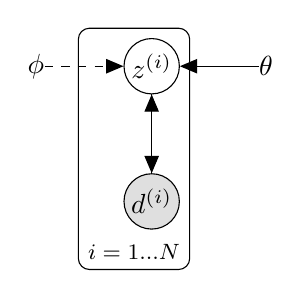
\begin{tikzpicture}[node distance = 1.5cm]
			
			
			\node[obs] (d) {$d^{(i)}$};
			
			\node[latent, above=of d] (z) {$z^{(i)}$};
			
			\node[const, right=of z] (th) {$\theta$} ;
			\node[const, left=of z] (ph) {$\phi$};
			
			
			\edge {z} {d};
			\edge {th} {z};
			\edge [dashed,bend left] {d} {z}
			\edge [dashed] {ph} {z}
			
			
			
			\plate {zd} {(z)(d)} {$i = 1...N$};
			
			\end{tikzpicture}
		\end{center}
		\caption{Graphical Model}
		\label{VAE}
	\end{figure}
	
	
	Discuss implications of plate difference? Discuss alternative approach with separate latent variables and/or noise for each word?\\ \\
	
	\subsection{Application-specific choices}
	
	For the encoder $q(z|x)$ and the decoder $p(x|z)$ we use fully connected neural networks. The prior $p(z)$ over the latent variables is a Multivariate Gaussian with diagonal covariance: $N(0,0.01*I)$. A smaller variance than the variance $I$, often used in VAE's, proved to be more effective. This is presumably because the KL divergence is less restrictive this way. 
	\\
	(need to show experiment for smaller KLD?)
	
	
	The output of the decoder $p(x|z)$ is modeled as a Multinomial distribution. An obvious choice for count data such as bag-of-words data might also be a Poisson distribution. However, this also models document length, something we are not necessarily interested in.  
	
	Even though we might not want to model document length, it might be informative for the topic. From that perspective, it makes sense not to normalize the input $X$. However, this requires the encoder to be able to generalize over different input scales, as opposed to working with normalized data. We therefore perform experiments with both approaches.
	
	Discuss how interpretable the lower bound is (or later?). 

	\subsection{Objective Function}
	
	In a VAE, the log-likelihood of a data point i, $\mathbf{x}$, is written as a sum of the lower bound and the KL divergence term between the true posterior $p(z|x)$ and the approximation $q(z|x)$, with $\theta$ the parameters of the model:
	
	\begin{align*}
	\log p(\mathbf{x}^{(i)}) = D_{KL}(q(\mathbf{z}^{(i)}|\mathbf{x}^{(i)}) || p(\mathbf{z}|\mathbf{x}^{(i)})) + \mathcal{L}(\mathbf{\theta}, \phi)
	\end{align*}
	
	We optimize the lower bound on the log-likelihood: 
	
	\begin{align}
	%\mathcal{L}(\mathbf{\theta}, \phi; \mathbf{d}^{(i)}) = 
	%\mathbf{E}_{q_\phi} (\mathbf{z}|\mathbf{d}^{(i)})}[-\log
	%q_\ph	i (\mathbf{z}| \mathbf{d}^{(i)})+\log
	%p_\theta(\mathbf{z}^{(i)}|\mathbf{d}^{(i)}]
	\end{align}
	
	which, using Bayes rule, we can express as:
	
	\begin{align}
	\mathcal{L}(\mathbf{\theta}, \phi; \mathbf{x}^{(i)}) = -D_{KL}(q_\phi (\mathbf{z}| \mathbf{x}^{(i)})||p_\theta (\mathbf{z})) + \mathbf{E}_{q_\phi(\mathbf{z}|\mathbf{x}^{(i)})}[\log p_\theta (\mathbf{x}^{(i)}|\mathbf{z})]
	\end{align}

	
	
	Still following Kingma and Welling \cite{kingma2013auto}, we can integrate the KL divergence analytically to obtain: \\
	

	\begin{align}
	- D_{KL}(q_\phi (\mathbf{z}| \mathbf{x}^{(i)}||p_\theta (\mathbf{z}| \mathbf{x}^{(i)})) = \frac{1}{2}\sum\limits_{j=1}^{J}\{1+\log \sigma_{\phi ,j}^2 - \mu_{\phi,j}^2 - \sigma_{\phi ,j}^2\}
	\end{align}
	
	Where the $\mathbf{\mu}_{\theta,j}$ and $\mathbf{\sigma}_{\theta,j}^2$ represent the $j$ -th mean and variance of the parametrized $q_\theta(\mathbf{z}|\mathbf{d})$.
	
	An obvious choice for modeling the output distribution for count data would be Poisson. However, this also models the length of a document, which we do not expect to be very relevant for the topic. Therefore we use Multinomial probability for each word $x_n^{i}$ in document $d^{i}$. This way, we have that
	
	\begin{align}
	\log p_{\theta}(d^{(i)}|z^{(i)}) = 
	\sum_{n=1}^N
	\sum_{k=1}^K x_k^{(in)} \log (y_k^{(in)})
	\end{align}
	Where $k$ is the index of the output unit.\\
	
	
	Using a SGVB estimator, our final objective function consists of the negative KL divergence and the reconstruction error:
	
	\begin{align}
	\mathcal{L}(\mathbf{\theta}, \phi; \mathbf{d}^{(i)}) = \frac{1}{2}\sum\limits_{j=1}^{J}\{1+\log \sigma_{\phi ,j}^2 - \mu_{\phi,j}^2 - \sigma_{\phi ,j}^2\} 
	+ \sum_{n=1}^N
	\sum_{k=1}^K x_k^{(in)} \log (y_k^{(in)})
	\end{align}
	
\section{Stick Breaking Topic VAE}
\subsection{Introduction}
One potential problem of a VAE is that the probability mass of the prior over the latent variables is centered around zero. Therefore, a non-centered distribution, such as in many binary latent variable models (e.g. LDA) might be might be more discriminative. As we have sparse data where data points (i.e. documents) frequently can be described by only a few of the used latent variables (roughly corresponding to topics), this seems particularly applicable to our application.  \\
The Beta distribution can not be used for SGVB as the inverse CDF is intractable. \\
Nalisnyck \& Smith use the Kumaraswami distribution, a close approximation to the Beta distribution with a tractable inverse CDF, to define a Stick-Breaking VAE. \\

\section{Random Projections}
Idea: use a random projection of all scarce words in the dataset as extra information for the encoder. This hardly adds computational complexity, but might still improve inference.

\section{Graph Convolutional Topic VAE}
Bag-of-words data can be seen as a bi-partite graph, which makes the work bij Kipf \& Welling very relevant.
\subsection{Graph Convolutions for SGVB Topic Modelling}
Describe the limitations our application provides for using graph convolutions.\\
Describe exactly how we use Graph Convolutions. The rest of the model does not change in comparison to earlier models, e.g. latent variable methods and accompanying objective functions(s).


\chapter{Experiments}
	\textit{Open question: How do we compare to e.g. Deep Exponential families if we don't use the same vocabulary size? Running Experiments with Deep Exponential Families myself is a lot of work and computation time and requires using good hyperparameters. One (mediocre) idea is to estimate the difference in model perplexity as a result of vocabulary reduction with the (theoretical and practical) results obtained by Kobayashi, or train one VAE model on the full vocabulary to obtain a good estimate for the difference. This last option will probably lead to numerical instability problems.}

	We ran experiments on the KOS and the NY Times datasets, freely available at UCI\footnote{https://archive.ics.uci.edu/ml/datasets/Bag+of+Words}. Both datasets contain only words that occur more than ten times in the whole dataset. The KOS dataset contains 3430 documents and has a vocabulary size of 6906. The dataset was split into 3300 training documents and 130 test documents. The NY times dataset consists of 300,000 documents and has a vocabulary size of 102,660 words. For the NY Times dataset, we only use words that occur over 3,000 times in the dataset. This makes training time and model evaluation a lot faster, as both scale approximately linearly with input dimensionality. Leaving out infrequent words only has a minor effect on the perplexity of bag-of-word topic model perplexity, mainly due to Zipf's law (Cite Kobayashi). For this dataset, a test set of 1,000 documents was used.
	\\
	For our experiments on KOS, we used one hidden layer of 400 units in the encoder and one hidden layer of 100 units in the decoder.  Using a more powerful decoder resulted in over-fitting on the train set. 
	\\
	Held-out perplexity was calculated for the test set as in e.g. (cite deep exponential families, welling, more?) by showing only half the words, randomly sampled, in each document to the encoder to obtain $\mathbf{z}$, identical to during training. The average per-word perplexity of the unseen words is then calculated under the word-probabilities predicted by the decoder.  Figure \ref{results_KOS} compares perplexities for KOS to LDA, as well as the achieved lower bound on the test set.
	\\
	
	
	\begin{tabular}{l|l|l|l}
		& VAE, unnormalized & VAE, normalized & LDA  \\
		\hline
		lower bound & & & - \\
		\hline
		perplexity & & & \\
		\label{results_KOS}
	\end{tabular}


\chapter{Discussion}
What are advantages/disadvantages of our method(s) compared to existing approaches?\\
How does our method compare to other methods as far as perplexity goes? Can we understand this?\\
For which purposes would we recommend (one of) our approaches, and why? \\
\section{Conclusion}
\section{Future Work}
\bibliography{ref}
\end{document}